\documentclass[../main.tex]{subfiles}
\begin{document}
\chapter{Casi d'uso}
\section{Catalogo dei casi d'uso}
\begin{tabularx}{150mm}{|c|X|}
    \hline
    \textbf{Codice caso d'uso}          & \textbf{Titolo} \\
    \hline
    UC001   &   Login alla piattaforma \\
    \hline
    UC002   &   Selezione dell'ambiente \\
    \hline
    UC003   &   Selezione della sessione di lavoro \\
    \hline
    UC004   &   Aggiunta di un dispositivo \\
    \hline
    UC005   &   Aggiunta di un link tra due dispositivi \\
    \hline
    UC006   &   Eliminazione di un elemento dal canvas \\
    \hline
    UC007   &   Configurazione di un dispositivo \\
    \hline
    UC008   &   Configurazione di un link \\
    \hline
    UC009   &   Deploy della topologia di rete \\ 
    \hline
    UC010   &   Apertura del terminale di un dispositivo \\
    \hline
    UC011   &   Creazione di una sessione di lavoro \\
    \hline
    UC012   &   Associazione di utenti a una sessione di lavoro \\
    \hline
    UC013   &   Generazione di un invite link per l'associazione degli utenti \\
    \hline
    UC014   &   Join di una sessione di lavoro tramite invite link \\
    \hline
    UC015   &   Logout di un utente \\
    \hline
\end{tabularx}
\newpage
\section{Diagramma dei casi d'uso}
\begin{figure}[H]
\centering
%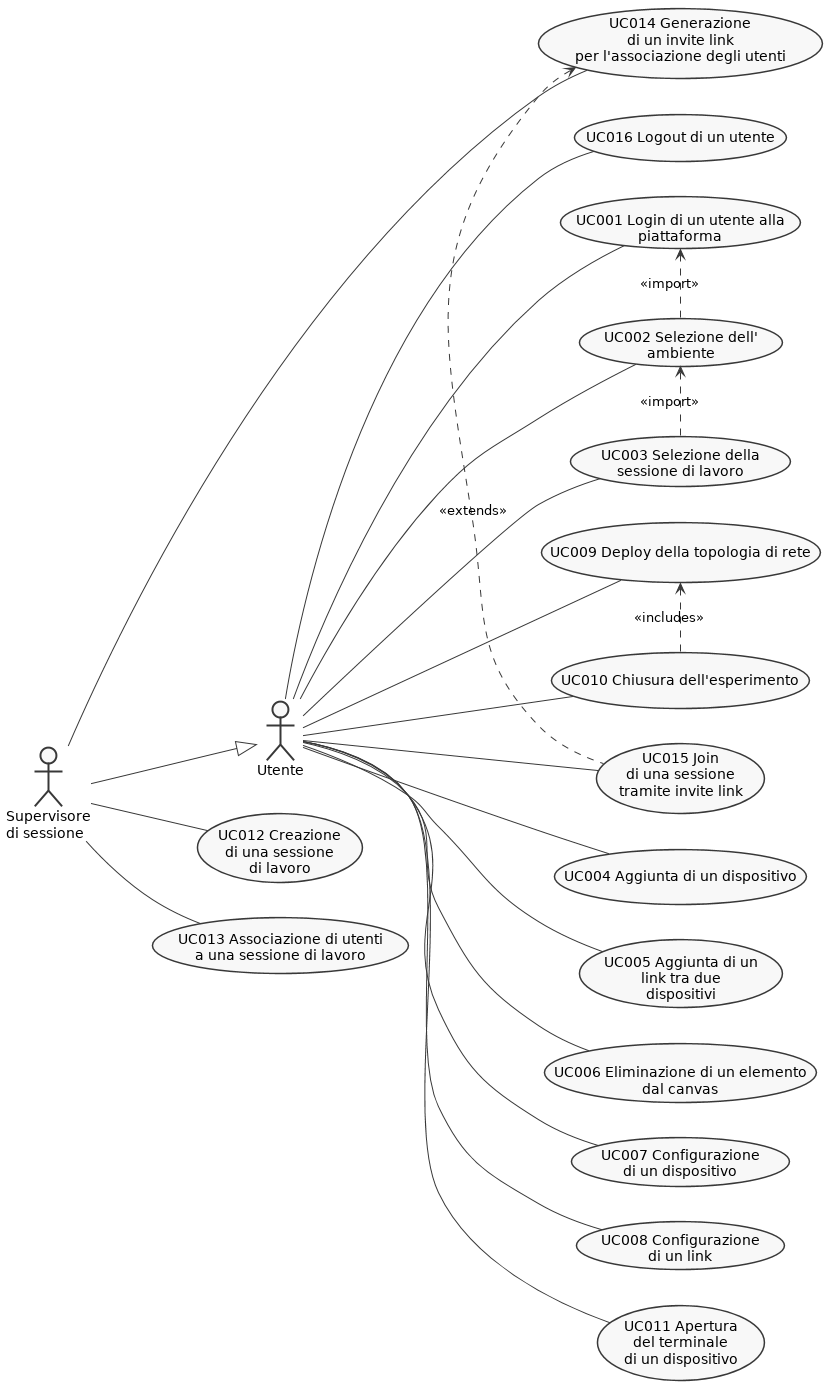
\includegraphics[height=21cm]{capitoli/diagramma-casi-d-uso.png}
\includesvg[svgpath=capitoli/, height=21cm, pretex=\tiny]{diagramma-casi-d-uso}
\end{figure}
\newpage
\section{Schede dei casi d'uso}
\subfile{capitoli/usecases/usecases.tex}
\end{document}
